% PosterAgent Course Report — upload this folder to Overleaf
% Option A: Upload paper/overleaf/ as a ZIP (New Project > Upload Project)
% Option B: In Overleaf, search Templates for "ICLR", then replace main.tex with this file

\documentclass{article}

\usepackage[margin=1in]{geometry}
\usepackage{times}
\usepackage{microtype}
\usepackage{graphicx}
\usepackage{booktabs}
\usepackage{amsmath,amssymb}
\usepackage{hyperref}
\usepackage{url}
\usepackage{xcolor}
\usepackage{enumitem}
\usepackage{caption}
\usepackage{subcaption}
\usepackage{algorithm}
\usepackage{algpseudocode}

\hypersetup{colorlinks=true, linkcolor=blue, citecolor=blue, urlcolor=blue}

\title{\textbf{PosterAgent: Training-Free Hierarchical Multi-Agent Optimization\\for Academic Poster Generation}}

\author{
  [Member 1 Name]\thanks{Student ID: [ID]. Email: [email@university.edu]} \and
  [Member 2 Name]\thanks{Student ID: [ID].} \and
  [Member 3 Name]\thanks{Student ID: [ID].} \and
  [Member 4 Name]\thanks{Student ID: [ID].}\\[0.5em]
  \textit{Computer Graphics, Spring 2026, Project 3}
}

\date{}

\begin{document}
\maketitle

\begin{abstract}
Academic posters remain a primary medium for communicating research at conferences, yet manual design is time-consuming and existing automation tools often produce posters with fragmented logic, poor figure readability, and rigid iteration schedules. We present \textbf{PosterAgent}, a \textbf{training-free hierarchical multi-agent framework} that transforms PDF research papers into publication-quality academic posters without fine-tuning any layout or vision model. Our system introduces: (1) a \textbf{logic-first content pipeline} with cross-section \emph{LogicPlan} and semantic dependency checks; (2) a \textbf{semantically assigned three-column academic layout} (25\%/50\%/25\%) with \textbf{content-level column balancing}; and (3) a \textbf{paper-native figure pipeline} that renders and role-crops PDF figures at panel boundaries to avoid mid-panel clipping. A \textbf{multi-metric adaptive controller} fuses semantic completeness, layout balance, and image--text match scores. On a \emph{Nature Methods} paper (GRASP), composite quality improves from \textbf{0.53 to 0.86} in three iterations. Code: \url{https://github.com/YOUR_USERNAME/poster-agent}.
\end{abstract}

\noindent\textbf{Keywords:} academic poster generation, multi-agent systems, document layout, figure extraction, LLM orchestration

\section{Introduction}
\label{sec:intro}

Conference posters condense long-form papers into a single visual narrative. Unlike slides, posters must satisfy \emph{information completeness}, \emph{logical coherence}, \emph{visual hierarchy}, and \emph{spatial efficiency} on a fixed canvas (typically 36$\times$24 inches). Researchers spend hours selecting figures, writing bullets, and balancing columns---tasks that are repetitive yet highly structured.

Recent work automates poster generation with large language models (LLMs). \textbf{Paper2Poster} uses Parser--Planner--Painter stages; \textbf{PosterForest} organizes content as a hierarchical tree; \textbf{GenPilot} applies error analysis to refine generation pipelines. These approaches share critical limitations:
\begin{enumerate}[leftmargin=*]
  \item \textbf{Logic fragmentation.} Section summaries are generated independently; Results may cite benchmarks never introduced in Methods.
  \item \textbf{Figure misuse.} Embedded PDF thumbnails are low-resolution; naive scaling either crops figures at arbitrary boundaries (``waist-cutting'') or shrinks multi-panel figures until labels become illegible.
  \item \textbf{Single-dimensional feedback.} Overflow detection alone cannot judge image--text alignment or column narrative balance.
  \item \textbf{Fixed iteration budgets.} Two-pass loops waste compute on easy papers and under-optimize hard ones.
\end{enumerate}

We address these gaps with \textbf{PosterAgent}: 15+ specialized agents over three data structures---\textbf{Raw Document Tree}, \textbf{Content Tree}, and \textbf{Poster Tree}. The system requires only an instruction-following LLM (DeepSeek-V4-Flash) and Python libraries (PyMuPDF, Pillow, Matplotlib, python-pptx)---\textbf{no model training}.

\paragraph{Contributions.}
\begin{enumerate}[label=\textbf{C\arabic*.}, leftmargin=*]
  \item \textbf{Logic-first multi-agent content generation} via \emph{LogicPlannerAgent}, \emph{logic\_links}, and \emph{SemanticCheckAgent}.
  \item \textbf{Semantically assigned three-column layout} (Introduction/Methods left, Results center 50\%, back matter right).
  \item \textbf{Section expander + column balancer} that adjusts text content, not line spacing, to equalize column heights.
  \item \textbf{Paper-native figure pipeline} with role-aware cropping (\texttt{intro}, \texttt{benchmark}, \texttt{structure}).
  \item \textbf{Multi-metric adaptive control} with outer semantic loop and inner overflow re-layout.
\end{enumerate}

We validate on \textbf{GRASP}~\citep{zhang2025grasp}, a 22-page \emph{Nature Methods} paper with multi-panel figures and DockQ benchmarks (Figure~\ref{fig:poster}).

\section{Related Work}
\label{sec:related}

\paragraph{Automated poster generation.}
Paper2Poster~\citep{paper2poster2024} pioneered Parser--Planner--Painter decomposition but lacks cross-section logic verification. PosterForest~\citep{posterforest2024} merges hierarchical trees with fixed iteration. Commercial templates ignore paper-aware parsing.

\paragraph{Document understanding.}
GROBID, Marker, and Docling extract structured text but do not reason about poster narrative. Our \emph{ParserAgent} renders figure pages at 220--240\,DPI and builds a scored \emph{FigureCatalog}.

\paragraph{Multi-agent orchestration.}
Generic frameworks (AutoGen, LangGraph) lack poster-specific typed interfaces. Our \emph{PosterErrorAnalyzer} routes overflow/sparsity to refiner, layout, or visual fixers---following GenPilot~\citep{genpilot2024} error-analysis principles.

\begin{table}[t]
  \centering
  \caption{Comparison with poster generation baselines.}
  \label{tab:compare}
  \small
  \begin{tabular}{lcccc}
    \toprule
    Method & Logic & Figures & Columns & Adaptive \\
    \midrule
    Paper2Poster & Partial & Embedded & Generic & Fixed 2-pass \\
    PosterForest & Tree merge & Limited & Static & Fixed \\
    Single LLM + PPTX & None & Manual & Template & Single shot \\
    \textbf{PosterAgent (Ours)} & \textbf{LogicPlan} & \textbf{Role crop} & \textbf{3-col semantic} & \textbf{Score threshold} \\
    \bottomrule
  \end{tabular}
\end{table}

\section{Method}
\label{sec:method}

\subsection{System Overview}

PosterAgent executes (Figure~\ref{fig:pipeline}):
\begin{enumerate}[leftmargin=*]
  \item \textbf{Parse} PDF $\rightarrow$ Raw Tree + figure catalog + tables.
  \item \textbf{Plan} LogicPlan (pipeline steps, validation chain).
  \item \textbf{Iterate} until composite score $\geq \tau$ (default 0.85):
  refine content $\rightarrow$ expand sections $\rightarrow$ enrich visuals $\rightarrow$ balance columns $\rightarrow$ layout $\rightarrow$ render $\rightarrow$ evaluate.
  \item \textbf{Output} best-iteration PNG/PPTX.
\end{enumerate}

Three-tree separation enables \textbf{targeted feedback}: semantic issues $\rightarrow$ Refiner; overflow $\rightarrow$ Layout with \texttt{height\_boost}; missing visuals $\rightarrow$ VisualAgent.

\begin{figure}[t]
  \centering
  \fbox{\parbox{0.92\linewidth}{\small
  \textbf{Pipeline:}\quad
  PDF $\rightarrow$ Parser $\rightarrow$ LogicPlanner $\rightarrow$ [\textbf{Loop}] Refiner $\rightarrow$ SectionExpander $\rightarrow$ VisualAgent $\rightarrow$ ColumnBalancer $\rightarrow$ Painter $\rightarrow$ SemanticCheck $\rightarrow$ Layout $\rightarrow$ Paint $\rightarrow$ ErrorAnalyzer $\rightarrow$ Balance $\rightarrow$ Commenter $\rightarrow$ Controller $\rightarrow$ Best PNG/PPTX
  }}
  \caption{PosterAgent multi-agent pipeline. SectionExpander and ColumnBalancer activate in three-column academic mode.}
  \label{fig:pipeline}
\end{figure}

\subsection{Logic-First Content Generation}

\emph{LogicPlannerAgent} outputs a \texttt{LogicPlan} \emph{before} refinement: \texttt{core\_problem}, \texttt{pipeline\_steps}, \texttt{validation\_chain}, \texttt{key\_terms}. \emph{RefinerAgent} preserves \texttt{logic\_links} (e.g., \texttt{Methods$\rightarrow$Results: benchmark validation}). \emph{SemanticCheckAgent} scores cross-section consistency ($\mathit{logic\_score}$).

\subsection{Section Expansion and Column Balancing}

\emph{SectionExpander} transforms flat sections into ORF3a-style panel stacks:
\begin{itemize}[leftmargin=*]
  \item \textbf{Results:} benchmark figure, structure figure, DockQ chart, key findings (4 panels).
  \item \textbf{Methods:} graph encoding + integration pipeline (2 panels).
  \item \textbf{Discussion:} Conclusions, Future Directions, Acknowledgements, References.
\end{itemize}

\emph{ColumnBalancer} estimates column height from layout plans and expands/trims bullet text (References, Future Work) or trims overflowing Results panels---\textbf{without} line-spacing distortion.

\subsection{Paper-Native Figure Pipeline}
\label{sec:figures}

Four stages address waist-cutting and illegible scaling:
\begin{enumerate}[label=\textbf{S\arabic*.}, leftmargin=*]
  \item \textbf{Page rendering:} \texttt{render\_figure\_focus\_panels()} at 240\,DPI with caption-aware bounds.
  \item \textbf{Role-aware cropping:} \texttt{split\_horizontal\_bands()} detects whitespace ($\geq$96.5\% white rows); outputs \texttt{fig\{N\}\_crop\_\{intro|benchmark|structure\}.png}.
  \item \textbf{Catalog assignment:} \texttt{figure\_curator} maps crops to panels by title semantics.
  \item \textbf{Display:} contain-mode paste (never cover-crop); up to 42\% panel height for paper figures.
\end{enumerate}

\subsection{Layout Engine}

\emph{GridLayoutEngine} uses 3600$\times$2400\,px canvas, \texttt{column\_fracs=(0.25, 0.50, 0.25)}. Title-driven routing assigns sections to narrative columns. Slack height goes to the \textbf{last section per column} to avoid inter-section voids. \texttt{panel\_stack} divides Results height among child panels (28/28/24/20\%).

\subsection{Multi-Metric Adaptive Control}

\begin{align}
  \mathit{semantic} &= 0.6 \cdot SC + 0.4 \cdot \mathit{logic\_score} \\
  \mathit{overall} &= 0.4 \cdot \mathit{semantic} + 0.35 \cdot LB + 0.25 \cdot ITM
\end{align}

$SC$ and $ITM$ come from \emph{CommenterAgent}; $LB$ from \emph{BalanceAgent} (alignment, whitespace, density, overflow). \emph{ControllerAgent} stops at $\mathit{overall} \geq 0.85$ or max 5 iterations, keeping the \textbf{best} iteration.

\section{Experimental Results}
\label{sec:experiments}

\subsection{Setup}

\textbf{Case study:} GRASP~\citep{zhang2025grasp}, 22 pages, multi-panel figures, DockQ tables. \textbf{Canvas:} 3600$\times$2400 landscape, three-column academic mode. \textbf{LLM:} DeepSeek-V4-Flash.

\subsection{Iterative Optimization (v16)}

Table~\ref{tab:scores} shows score progression over three iterations:

\begin{table}[t]
  \centering
  \caption{Composite score progression on GRASP (v16 run).}
  \label{tab:scores}
  \small
  \begin{tabular}{cccccc}
    \toprule
    Iter & logic & LB & ITM & semantic & \textbf{Overall} \\
    \midrule
    1 & 0.65 & 0.786 & 0.20 & 0.50 & \textbf{0.525} \\
    2 & 0.60 & 0.825 & 0.60 & 0.54 & \textbf{0.655} \\
    3 & 0.90 & 0.814 & 0.95 & 0.84 & \textbf{0.858} \\
    \bottomrule
  \end{tabular}
\end{table}

ITM improved $0.20 \rightarrow 0.95$, confirming figure assignment as the primary early bottleneck. Controller converged at iteration~3 ($\tau=0.85$).

\subsection{Figure Crop Ablation}

\begin{table}[t]
  \centering
  \caption{Figure readability ablation on GRASP.}
  \label{tab:crop}
  \small
  \begin{tabular}{lccc}
    \toprule
    Configuration & Fig.2 readable & Fig.3 readable & Mid-panel clip \\
    \midrule
    Full focus figures & No & No & No \\
    Role-aware crops & \textbf{Yes} & \textbf{Yes} & \textbf{No} \\
    \bottomrule
  \end{tabular}
\end{table}

After 12+ engineering iterations (v8--v19), the final poster (\textbf{v19\_crop}) combines panel-stack layout, painter attach fix, and role-aware cropping.

\begin{figure}[t]
  \centering
  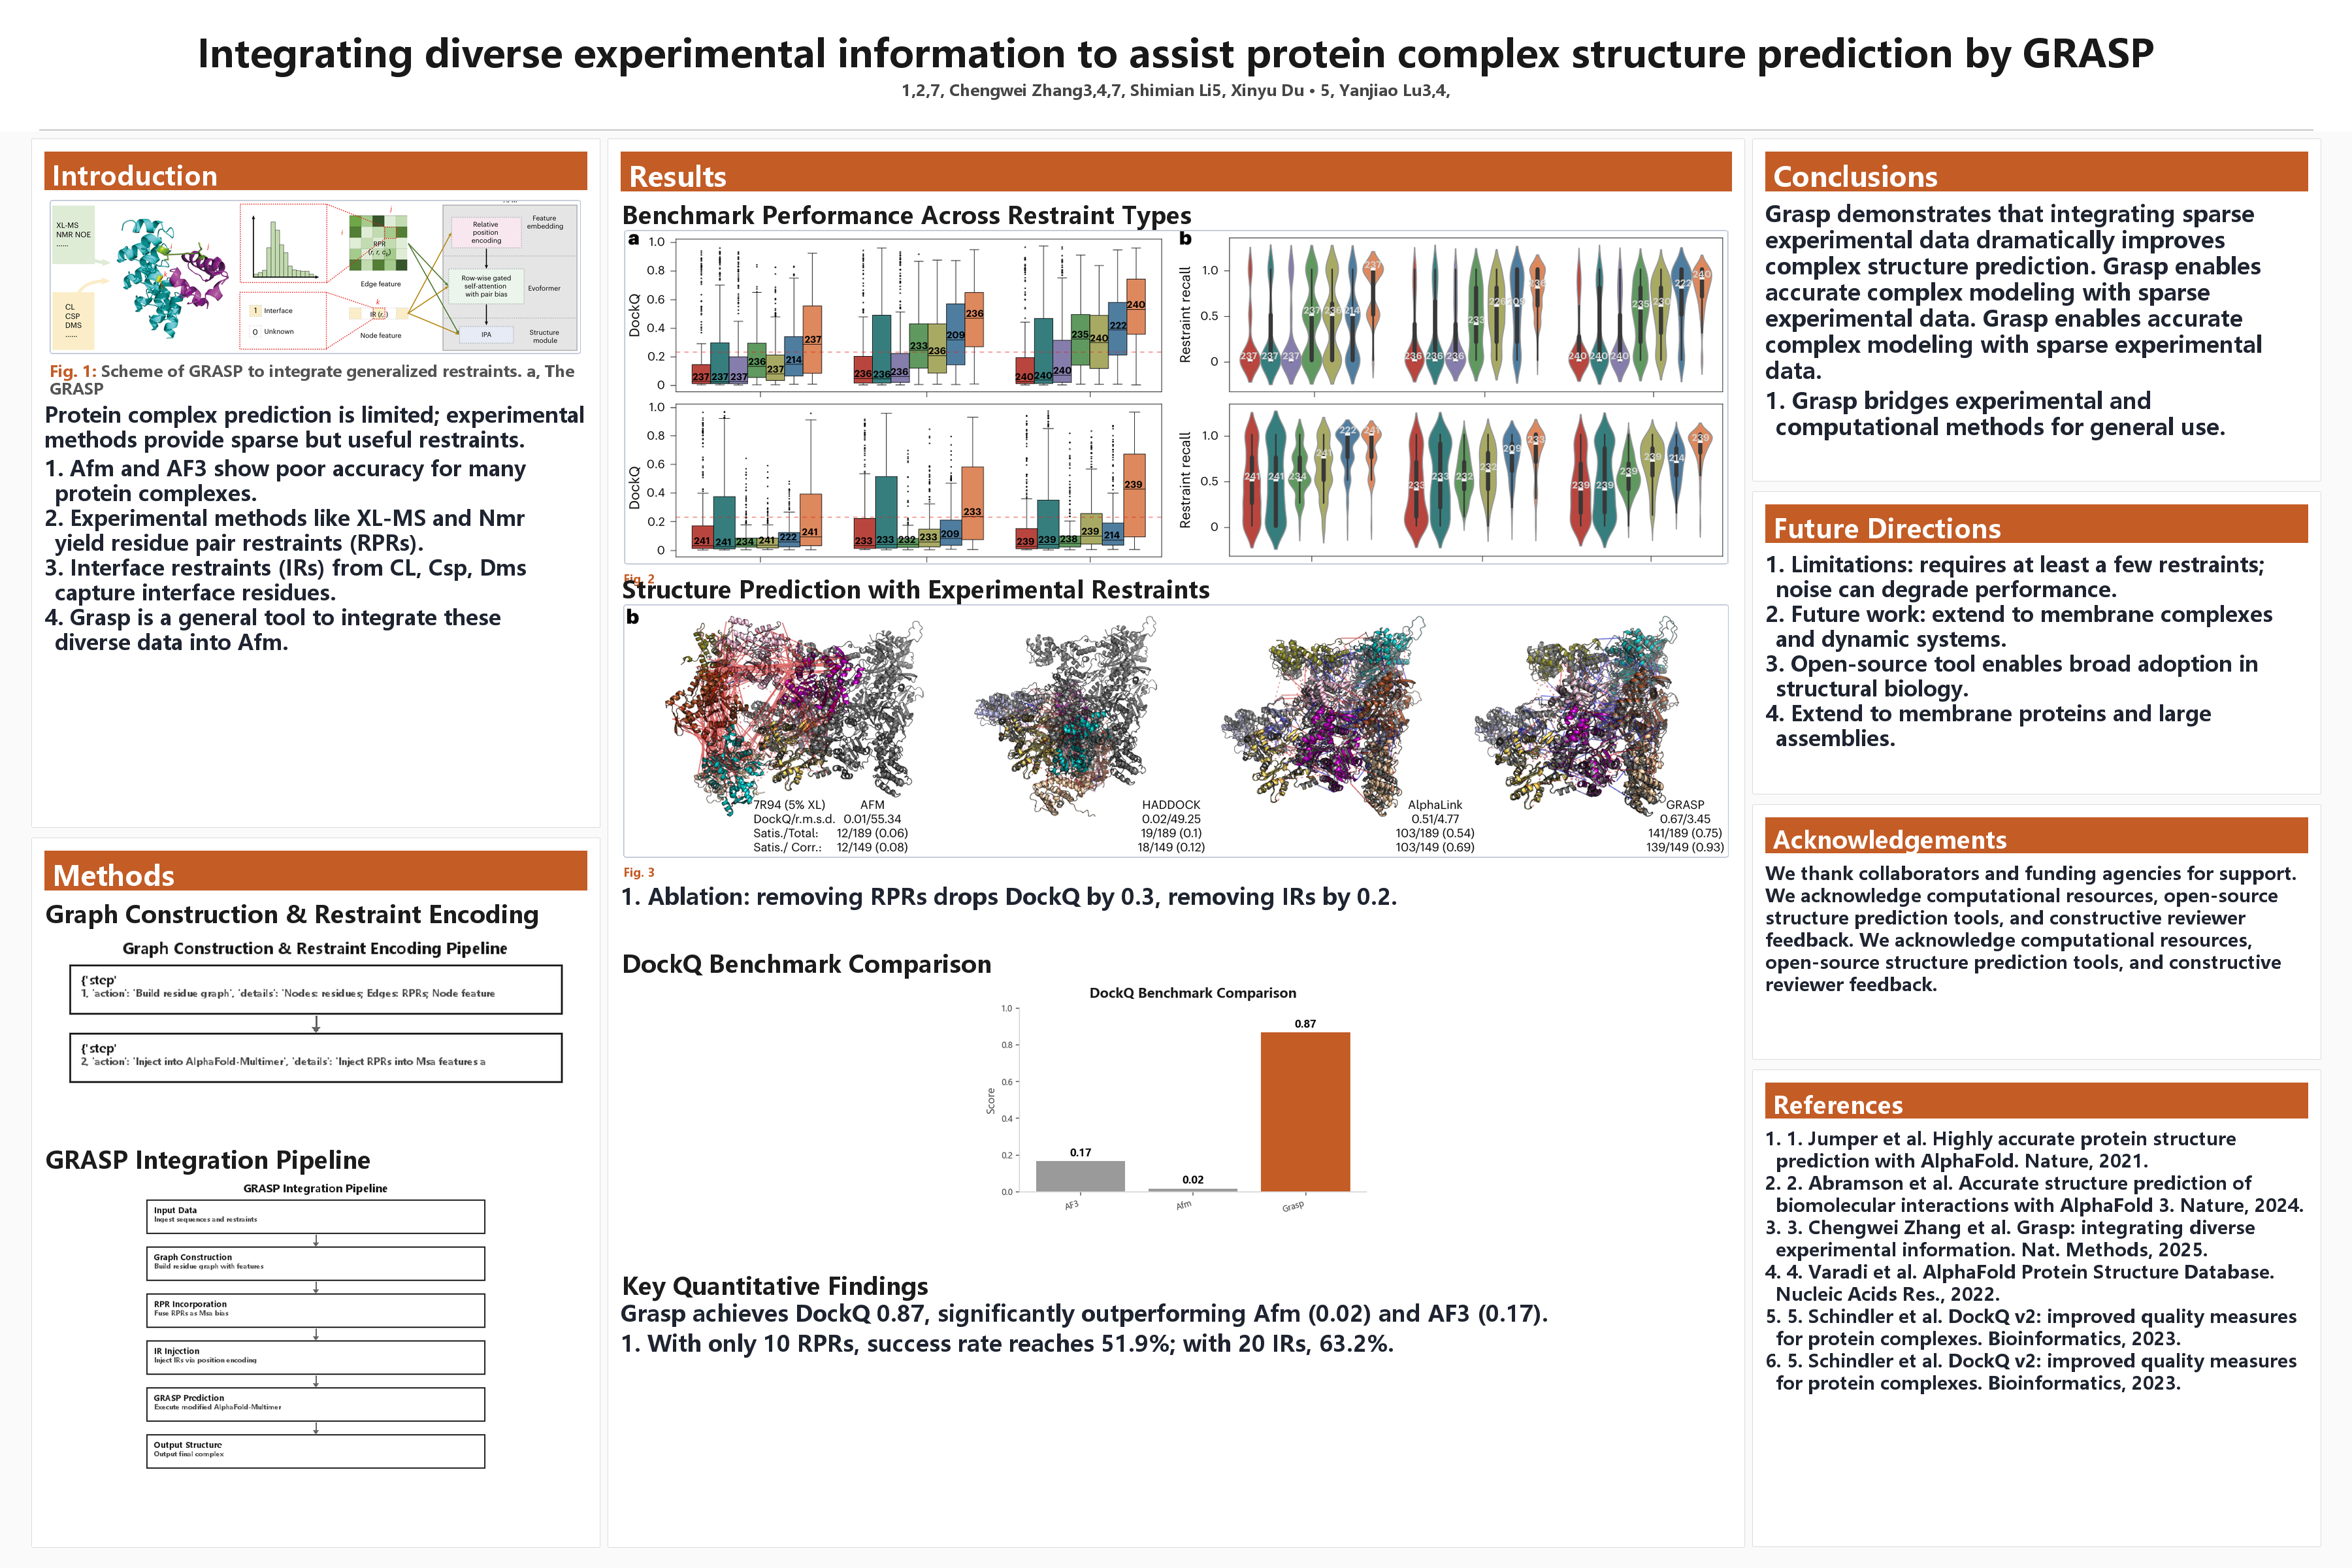
\includegraphics[width=\linewidth]{figures/poster_final.png}
  \caption{Final poster generated by PosterAgent on GRASP (\texttt{s41592\_02820\_v19\_result.png}). Three-column layout with cropped benchmark/structure figures and DockQ bar chart.}
  \label{fig:poster}
\end{figure}

\subsection{Efficiency and Limitations}

Adaptive termination used 3 iterations vs.\ a fixed 5-pass budget (40\% reduction). Re-render from saved JSON completes in ${\sim}$100\,s.

\textbf{Limitations:} LLM quality variance; whitespace-band cropping assumes horizontal panel separation; evaluation partly relies on LLM self-judgment.

\section{Conclusion}

We presented PosterAgent, a training-free hierarchical multi-agent system for academic poster generation. Logic-first refinement, semantic three-column layout, content-level column balancing, and role-aware figure cropping produce posters that are logically coherent, visually balanced, and figure-readable. On GRASP, quality improved from 0.53 to 0.86 in three iterations.

Future work: human expert evaluation, learned panel segmentation, interactive crop editing, and 60-paper benchmark.

\section*{Acknowledgments}
We thank the Computer Graphics course staff. GRASP paper and figures are courtesy of Zhang et al.~\citep{zhang2025grasp}. We cite PyMuPDF~\citep{pymupdf}, DeepSeek API, and public agent-framework literature.

% Required: group division of labor
\section*{Group Members and Division of Labor}
\begin{table}[h]
  \centering
  \small
  \begin{tabular}{llp{7.5cm}}
    \toprule
    Name & Student ID & Division of Labor \\
    \midrule
    [Member 1] & [ID] & System architecture; Parser/Refiner/LogicPlanner; pipeline \\
    [Member 2] & [ID] & Layout engine; three-column mode; column balancer \\
    [Member 3] & [ID] & Figure pipeline; Painter/Renderer; visual QA \\
    [Member 4] & [ID] & Evaluation agents; experiments; report and demo \\
    \bottomrule
  \end{tabular}
\end{table}

\bibliographystyle{plain}
\bibliography{references}

\end{document}
